% \section{Proof of Lemma~\ref{lem:measuresets}}\label{app:measuresets}
\begin{proof}
Let
\begin{equation}
f_\nsamps (\param) = \sum_{\iparam=1}^{\nsamps} \frac{\eta_\nsamps (\VV^{(\iparam)}) }{\mu (\VV^{(\iparam)})} \Chi_{\VV^{(\iparam)}} (\param).
\end{equation}
Then, for any $A\in\BB_\pspace$, define
\begin{equation}
\eta (A) = \int_A f_\nsamps (\param) \, d\mu.
\end{equation}
We verify that $\eta$ is a probability measure on $(\pspace, \BB_\pspace)$ and that $\eta(A) = \eta_\nsamps(A) \; \forall \; A\in\BB_{\pspace, \nsamps}$ below:
\begin{itemize}
\item[(i)][Positive]
Let $A\in \BB_{\pspace}$.
\begin{equation*}
\begin{split}
\eta (A) &= \int_A f_\nsamps (\param) \, d\mu \\
&=  \int \Chi_A \sum_{\iparam=1}^{\nsamps} \frac{\eta_\nsamps (\VV^{(\iparam)}) }{\mu (\VV^{(\iparam)})} \Chi_{\VV^{(\iparam)}} (\param) \, d\mu \\
&= \sum_{\iparam=1}^{\nsamps} \left ( \frac{\eta_\nsamps (\VV^{(\iparam)}) }{\mu (\VV^{(\iparam)})} \int \Chi_{A\cap\VV^{(\iparam)}} (\param) \, d\mu \right ) \\
&= \sum_{\iparam=1}^{\nsamps} \left ( \frac{\eta_\nsamps (\VV^{(\iparam)}) }{\mu (\VV^{(\iparam)})} \mu\left (A\cap\VV^{(\iparam)}\right ) \right ) \geq 0
\end{split}
\end{equation*}

\item[(ii)][Definite]
\begin{equation*}
\eta (\nullset) = \int_\nullset f_\nsamps (\param) \, d\mu =\int \Chi_\nullset f_\nsamps (\param) \, d\mu = \mu(\nullset) = 0
\end{equation*}

\item[(iii)][Countably Additive]
Let $\set{A_k}_{k=1}^{\infty} \subset \BB_{\pspace}$.
\begin{equation*}
\begin{split}
\eta (\cup_k A_k) &= \int_{\cup_k A_k} f_\nsamps (\param) \, d\mu
= \int \Chi_{\cup_k A_k} f_\nsamps (\param) \, d\mu \\
&= \int \left( \sum_k \Chi_{A_k} \right ) f_\nsamps (\param) \, d\mu
=   \sum_k \int \Chi_{A_k} f_\nsamps (\param) \, d\mu \\
&=   \sum_k \int_{A_k} f_\nsamps (\param) \, d\mu = \sum_k \eta(A_k)
\end{split}
\end{equation*}


\noindent Finally, let $A\in\BB_{\pspace, \nsamps}\subset \BB_\pspace$.
Then there exists some $\iparam^* \in \set{1,2, \cdots, \nsamps}$ such that $\VV^{(\iparam^*)} = A$.
We have that
\begin{equation*}
\begin{split}
\eta (A) &= \int_A f_\nsamps (\param) \, d\mu
=  \int \sum_{\iparam=1}^{\nsamps} \left ( \frac{\eta_\nsamps (\VV^{(\iparam)}) }{\mu (\VV^{(\iparam)})} \Chi_{\VV^{(\iparam)}}\right ) \Chi_{\VV^{(\iparam^*)}} \, d\mu \\
&= \int \frac{\eta_\nsamps (\VV^{(\iparam^*)}) }{\mu (\VV^{(\iparam^*)})} \Chi_{\VV^{(\iparam^*)}} \, d\mu
= \frac{\eta_\nsamps (\VV^{(\iparam^*)}) }{\mu (\VV^{(\iparam^*)})} \mu (\VV^{(\iparam^*)}) \\
&= \eta_\nsamps (\VV^{(\iparam^*)}) = \eta_\nsamps (A).
\end{split}
\end{equation*}

\end{itemize}
\end{proof}

%%%%%%%%%%%%
\section{Alternative Perspective on SIP Solutions in Example\ref{subsec:pde-example}}
To further underscore the impact of incorporating the extra dimension of information in the data space and the impact it has on the reduction of uncertainty, we turn the reader's attention to Fig.~\ref{fig:pde-highd-2d-scatter}.
Recall from \ref{subsec:pde-example} that two maps were used to solve the SIP: $\qoi^{1D}$ and $\qoi^{2D}$, and MUD points were shown for twenty realizations of noise for each in Figure~\ref{fig:pde-convergence}.
In this figure, we use the updated densities from a solution to the SIP from each of $\qoi^{1D}$ and $\qoi^{2D}$ to give an alternative view to that in \ref{fig:pde-convergence} of the feasible region in $\pspace$.
We normalize our evaluations of the ratio of observed to predicted densities and plot the samples that exceed two thresholds, numerical zero (left), and $1/N$ (right) to give some sense of samples that may come from accept/reject algorithms (since our initial was uniform).

Both scatter-plots exhibit the same geometry, appearing to trace a band through the parameter space.
Fundamentally, at first glance at the left figure, it is already apparent that half of $\pspace$ has been ruled out, and that the correlation structure between the two knots has been discovered.
The samples from $\qoi^{2D}$, however, cluster more tightly around the optimal samples (the ``projection'' here refers to the sample which minimizes the 2-norm to the noiseless data).
The incorporation of two directions instead of one whittles away more of the parameter space as being less relatively likely.
If we were to perform accept/reject, the resulting set would be fairly well constrained to the upper-lefthand corner of the two-dimensional parameter space.

\begin{figure}[htbp]
\centering
  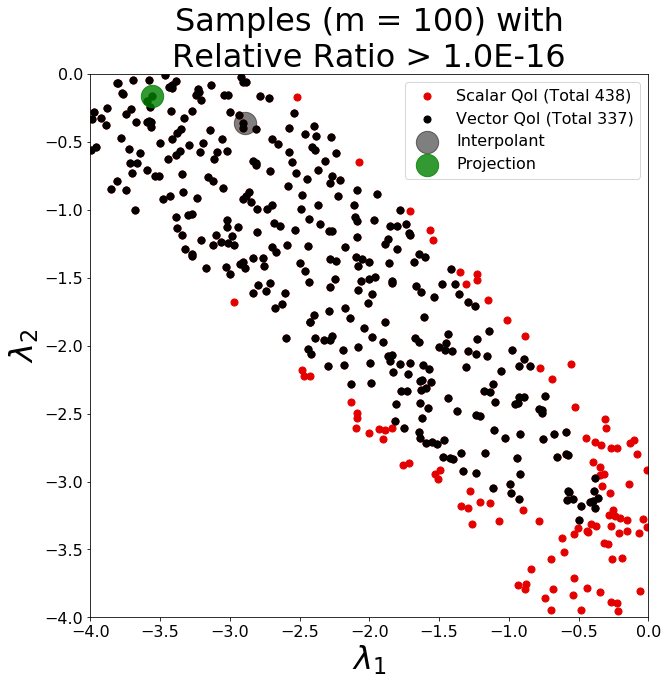
\includegraphics[width=0.45\linewidth]{figures/pde-highd/pde-highd_update_scatter_D2_t1-0E-16.png}
  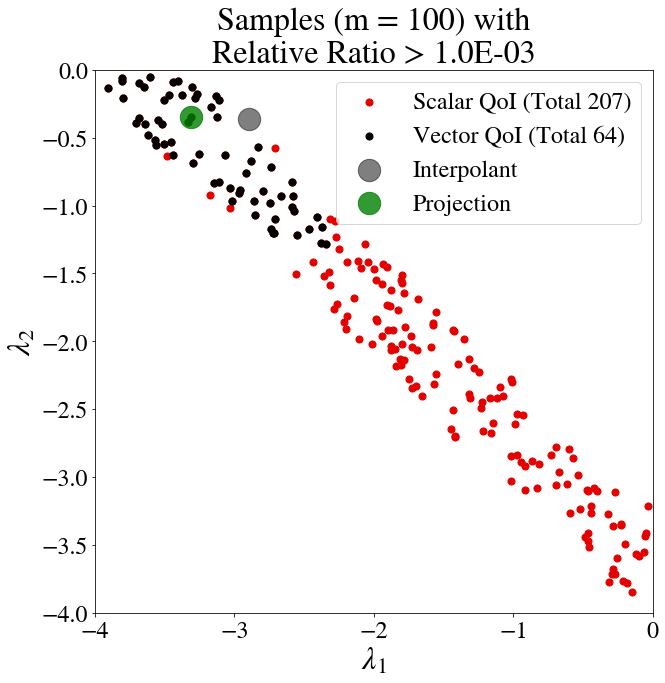
\includegraphics[width=0.45\linewidth]{figures/pde-highd/pde-highd_update_scatter_D2_t1-0E-03.png}
\caption{
100 measurements
}
\label{fig:pde-highd-2d-scatter}
\end{figure}

%%%%%%%%%%%%


We solve our SIP for twenty different realizations of noise to pollute our hundred measurements, and show the resulting solutions for the first twenty and all hundred being used to construct the vector--valued map.
The resulting functions that are induced by these MUD points are shown in Fig.~\ref{fig:pde-highd-2d-vector-mud}, and we note that solutions are no longer are considering the possibility of the minimum value of $g$ being at the wrong knot point as we saw in Fig.~\ref{fig:pde-highd-2d-scalar-mud}, even when only twenty total data points are used to construct $Q$.
By the time all hundred measurements are incorporated, the MUD solutions appear to be tracing out curves between the projection function and the interpolant function, a far more accurate set of predictions than those from the scalar--valued map (see \ref{fig:pde-highd-2d-scalar-mud}).

\begin{figure}[htbp]
\centering
  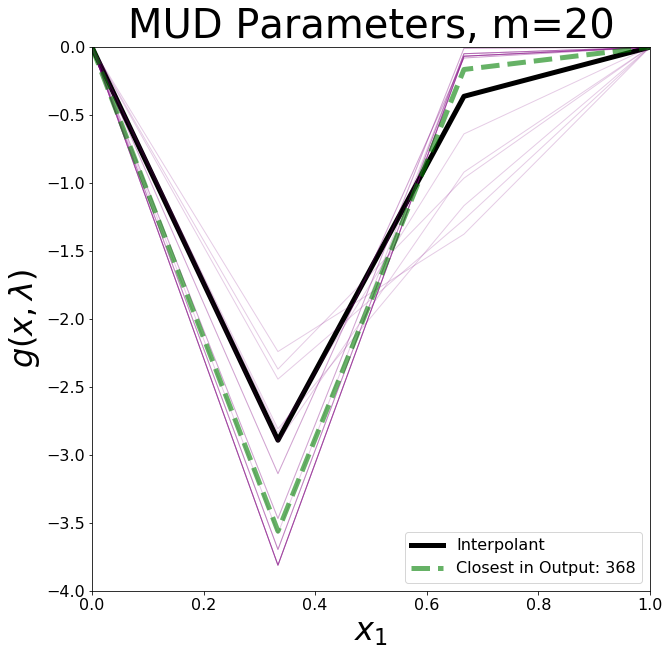
\includegraphics[width=0.6\linewidth]{figures/pde-highd/pde-highd_pair_D2-2_m20.png}
  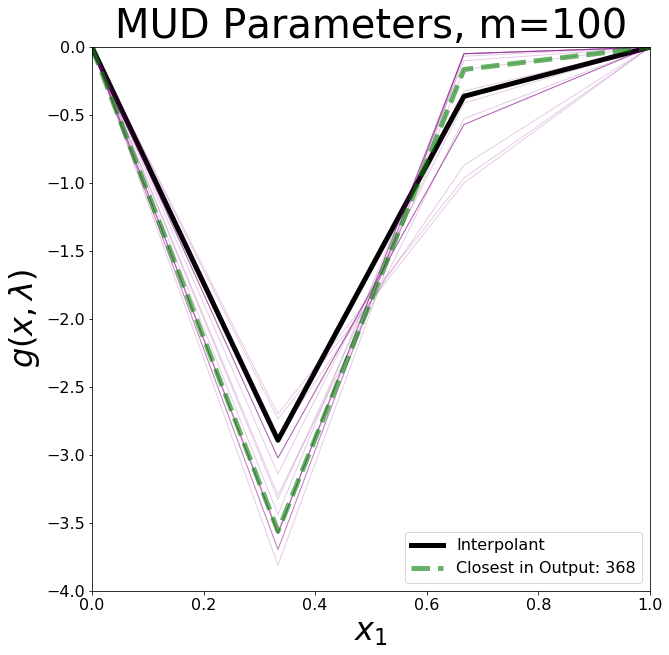
\includegraphics[width=0.6\linewidth]{figures/pde-highd/pde-highd_pair_D2-2_m100.png}
\caption{
(Top): When vectorizing our QoI map, we find that we are able to achieve more accuracy with fewer measurements. Here, we see far less variation in MUD solutions than in the bottom of Fig.~\ref{fig:pde-highd-2d-scalar-mud}.
(Bottom): When all 100 measurements are incorporated
}
\label{fig:pde-highd-2d-vector-mud}
\end{figure}

How we incorporate the available data has a dramatic impact on our ability to reduce uncertainty in the parameter space.
We attempt to illustrate this by requesting the reader juxtapose figures of the initial samples in \ref{fig:pde-highd-initial-2d} to those in \ref{fig:pde-highd-2d-scalar-mud} and \ref{fig:pde-highd-2d-vector-mud}.
To better quantify the differences between the two types of maps, it is more rigorous to study how close we are to $g$ (in function space).
Since the approximation $\hat{g}$ that arises from evaluating the MUD point is piecewise-linear, and $g$ is continuous, we use the knot points and the trapezoidal rule to approximate the $L^2$ norm of $\abs{g - \hat{g}}$ (using {\tt scipy}), and plot the resulting histograms for the scalar- and vector-valued $\param$s whose relative ratios exceeded a threshold, and compare them against samples from the initial density, and show the result in Figure~\ref{fig:pde-highd-2d-hist}.


\begin{figure}[htbp]
\centering
  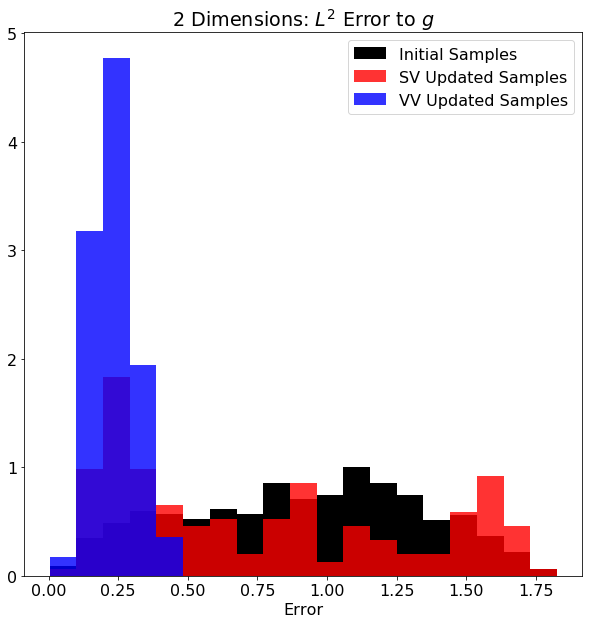
\includegraphics[width=0.675\linewidth]{figures/pde-highd/pde-highd_hist_D2_t5-0E-01}
\caption{
Histograms comparing initial samples with the highest probabilities (relative ratio $> 0.5$).
}
\label{fig:pde-highd-2d-hist}
\end{figure}

In \ref{fig:pde-highd-2d-hist}, the histograms have been normalized for comparison, and while the scalar--valued map still does reduce the uncertainty that we started with in our initial density, the vector--valued map is considerably more accurate.
The multi-modal nature of the scalar--valued histogram plot shows a lack of resolution that is not experienced at all by the vector--valued solution.
Both QoI maps solve a stochastic inverse problem, but the latter is more respectful of the geometry of the response surface, and so is able to learn significantly more, and bring us modelers far closer to the true function $g$.
The multi-modal density of probable samples corresponds to the two types of solutions we saw in Figure~\ref{fig:pde-highd-2d-scalar-mud}, but we are after a single parameter estimate of truth.
